\chapter{Case study: data structure selection}

\section{Word frequency analysis}
\label{analysis}

As usual, you should at least attempt the following exercises
before you read my solutions.

\begin{ex}
Write a program that reads a file, breaks each line into
words, strips whitespace and punctuation from the words, and
converts them to lowercase.

\index{string module}
\index{module!string}

Hint: The {\tt string} module provides strings named {\tt whitespace},
which contains space, tab, newline, etc., and {\tt
  punctuation} which contains the punctuation characters.  Let's see
if we can make Python swear:

\beforeverb
\begin{verbatim}
>>> import string
>>> print string.punctuation
!"#$%&'()*+,-./:;<=>?@[\]^_`{|}~
\end{verbatim}
\afterverb
%
Also, you might consider using the string methods {\tt strip},
{\tt replace} and {\tt translate}.

\index{strip method}
\index{method!strip}
\index{replace method}
\index{method!replace}
\index{translate method}
\index{method!translate}

\end{ex}


\begin{ex}

\index{Project Gutenberg}

Go to Project Gutenberg (\url{gutenberg.net}) and download 
your favorite out-of-copyright book in plain text format.

\index{plain text}
\index{text!plain}

Modify your program from the previous exercise to read the book
you downloaded, skip over the header information at the beginning
of the file, and process the rest of the words as before.

Then modify the program to count the total number of words in
the book, and the number of times each word is used.

\index{word frequency}
\index{frequency!word}

Print the number of different words used in the book.  Compare
different books by different authors, written in different eras.
Which author uses the most extensive vocabulary?
\end{ex}


\begin{ex}
Modify the program from the previous exercise to print the
20 most frequently-used words in the book.
\end{ex}


\begin{ex}
Modify the previous program to read a word list (see
Section~\ref{wordlist}) and then print all the words in the book that
are not in the word list.  How many of them are typos?  How many of
them are common words that {\em should} be in the word list, and how
many of them are really obscure?
\end{ex}


\section{Random numbers}

\index{random number}
\index{number, random}
\index{deterministic}
\index{pseudorandom}

Given the same inputs, most computer programs generate the same
outputs every time, so they are said to be {\bf deterministic}.
Determinism is usually a good thing, since we expect the same
calculation to yield the same result.  For some applications, though,
we want the computer to be unpredictable.  Games are an obvious
example, but there are more.

Making a program truly nondeterministic turns out to be not so easy,
but there are ways to make it at least seem nondeterministic.  One of
them is to use algorithms that generate {\bf pseudorandom} numbers.
Pseudorandom numbers are not truly random because they are generated
by a deterministic computation, but just by looking at the numbers it
is all but impossible to distinguish them from random.

\index{random module}
\index{module!random}

The {\tt random} module provides functions that generate
pseudorandom numbers (which I will simply call ``random'' from
here on).

\index{random function}
\index{function!random}

The function {\tt random} returns a random float
between 0.0 and 1.0 (including 0.0 but not 1.0).  Each time you
call {\tt random}, you get the next number in a long series.  To see a
sample, run this loop:

\beforeverb
\begin{verbatim}
import random

for i in range(10):
    x = random.random()
    print x
\end{verbatim}
\afterverb
%
The function {\tt randint} takes parameters {\tt low} and
{\tt high} and returns an integer between {\tt low} and
{\tt high} (including both).

\index{randint function}
\index{function!randint}

\beforeverb
\begin{verbatim}
>>> random.randint(5, 10)
5
>>> random.randint(5, 10)
9
\end{verbatim}
\afterverb
%
To choose an element from a sequence at random, you can use
{\tt choice}:

\index{choice function}
\index{function!choice}

\beforeverb
\begin{verbatim}
>>> t = [1, 2, 3]
>>> random.choice(t)
2
>>> random.choice(t)
3
\end{verbatim}
\afterverb
%
The {\tt random} module also provides functions to generate
random values from continuous distributions including
Gaussian, exponential, gamma, and a few more.

\begin{ex}

\index{histogram!random choice}

Write a function named \verb"choose_from_hist" that takes
a histogram as defined in Section~\ref{histogram} and returns a 
random value from the histogram, chosen with probability
in proportion to frequency.  For example, for this histogram:

\beforeverb
\begin{verbatim}
>>> t = ['a', 'a', 'b']
>>> h = histogram(t)
>>> print h
{'a': 2, 'b': 1}
\end{verbatim}
\afterverb
%
your function should {\tt 'a'} with probability $2/3$ and \verb"'b'"
with probability $1/3$.
\end{ex}


\section{Word histogram}

Here is a program that reads a file and builds a histogram of the
words in the file:

\index{histogram!word frequencies}

\beforeverb
\begin{verbatim}
import string

def process_file(filename):
    h = dict()
    fp = open(filename)
    for line in fp:
        process_line(line, h)
    return h

def process_line(line, h):
    line = line.replace('-', ' ')
    
    for word in line.split():
        word = word.strip(string.punctuation + string.whitespace)
        word = word.lower()

        h[word] = h.get(word, 0) + 1

hist = process_file('emma.txt')
\end{verbatim}
\afterverb
%
This program reads {\tt emma.txt}, which contains the text of {\em
  Emma} by Jane Austen.

\index{Austin, Jane}

\verb"process_file" loops through the lines of the file,
passing them one at a time to \verb"process_line".  The histogram
{\tt h} is being used as an accumulator.

\index{accumulator!histogram}
\index{traversal}

\verb"process_line" uses the string method {\tt replace} to replace
hyphens with spaces before using {\tt split} to break the line into a
list of strings.  It traverses the list of words and uses {\tt strip}
and {\tt lower} to remove punctuation and convert to lower case.  (It
is a shorthand to say that strings are ``converted;'' remember that
string are immutable, so methods like {\tt strip} and {\tt lower}
return new strings.)

Finally, \verb"process_line" updates the histogram by creating a new
item or incrementing an existing one.

\index{update!histogram}

To count the total number of words in the file, we can add up
the frequencies in the histogram:

\beforeverb
\begin{verbatim}
def total_words(h):
    return sum(h.values())
\end{verbatim}
\afterverb
%
The number of different words is just the number of items in
the dictionary:

\beforeverb
\begin{verbatim}
def different_words(h):
    return len(h)
\end{verbatim}
\afterverb
%
Here is some code to print the results:

\beforeverb
\begin{verbatim}
print 'Total number of words:', total_words(hist)
print 'Number of different words:', different_words(hist)
\end{verbatim}
\afterverb
%
And the results:

\beforeverb
\begin{verbatim}
Total number of words: 161073
Number of different words: 7212
\end{verbatim}
\afterverb
%

\section{Most common words}

\index{DSU pattern}
\index{pattern!DSU}

To find the most common words, we can apply the DSU pattern;
\verb"most_common" takes a histogram and returns a list of
word-frequency tuples, sorted in reverse order by frequency:

\beforeverb
\begin{verbatim}
def most_common(h):
    t = []
    for key, value in h.items():
        t.append((value, key))

    t.sort(reverse=True)
    return t
\end{verbatim}
\afterverb
%
Here is a loop that prints the ten most common words:

\beforeverb
\begin{verbatim}
t = most_common(hist)
print 'The most common words are:'
for freq, word in t[0:10]:
    print word, '\t', freq
\end{verbatim}
\afterverb
%
And here are the results from {\em Emma}:

\beforeverb
\begin{verbatim}
The most common words are:
to      5242
the     5204
and     4897
of      4293
i       3191
a       3130
it      2529
her     2483
was     2400
she     2364
\end{verbatim}
\afterverb
%

\section{Optional parameters}

\index{optional parameter}
\index{parameter!optional}

We have seen built-in functions and methods that take a variable
number of arguments.  It is possible to write user-defined functions
with optional arguments, too.  For example, here is a function that
prints the most common words in a histogram

\beforeverb
\begin{verbatim}
def print_most_common(hist, num=10)
    t = most_common(hist)
    print 'The most common words are:'
    for freq, word in t[0:num]:
        print word, '\t', freq
\end{verbatim}
\afterverb

The first parameter is required; the second is optional.
The {\bf default value} of {\tt num} is 10.

\index{default value}
\index{value!default}

If you only provide one argument:

\beforeverb
\begin{verbatim}
print_most_common(hist)
\end{verbatim}
\afterverb

{\tt num} gets the default value.  If you provide two arguments:

\beforeverb
\begin{verbatim}
print_most_common(hist, 20)
\end{verbatim}
\afterverb

{\tt num} gets the value of the argument instead.  In other
words, the optional argument {\bf overrides} the default value.

\index{override}

If a function has both required and optional parameters, all
the required parameters have to come first, followed by the
optional ones.


\section{Dictionary subtraction}

\index{dictionary!subtraction}
\index{subtraction!dictionary}

Finding the words from the book that are not in the word list
from {\tt words.txt} is a problem you might recognize as set
subtraction; that is, we want to find all the words from one
set (the words in the book) that are not in another set (the
words in the list).

{\tt subtract} takes dictionaries {\tt d1} and {\tt d2} and returns a
new dictionary that contains all the keys from {\tt d1} that are not
in {\tt d2}.  Since we don't really care about the values, we
set them all to None.

\beforeverb
\begin{verbatim}
def subtract(d1, d2):
    res = dict()
    for key in d1:
        if key not in d2:
            res[key] = None
    return res
\end{verbatim}
\afterverb
%
To find the words in the book that are not in {\tt words.txt},
we can use \verb"process_file" to build a histogram for
{\tt words.txt}, and then subtract:

\beforeverb
\begin{verbatim}
words = process_file('words.txt')
diff = subtract(hist, words)

print "The words in the book that aren't in the word list are:"
for word in diff.keys():
    print word,
\end{verbatim}
\afterverb
%
Here are some of the results from {\em Emma}:

\beforeverb
\begin{verbatim}
The words in the book that aren't in the word list are:
 rencontre jane's blanche woodhouses disingenuousness 
friend's venice apartment ...
\end{verbatim}
\afterverb
%
Some of these words are names and possessives.  Others, like
``rencontre,'' are no longer in common use.  But a few are common
words that should really be in the list!

\begin{ex}

\index{set}
\index{type!set}

Python provides a data structure called {\tt set} that provides many
common set operations.  Read the documentation at
\url{docs.python.org/lib/types-set.html} and write a program
that uses set subtraction to find words in the book that are not in
the word list.
\end{ex}


\section{Random words}
\label{randomwords}

\index{histogram!random choice}

To choose a random word from the histogram, the simplest algorithm
is to build a list with multiple copies of each word, according
to the observed frequency, and then choose from the list:

\beforeverb
\begin{verbatim}
def random_word(h):
    t = []
    for word, freq in h.items():
        t.extend([word] * freq)

    return random.choice(t)
\end{verbatim}
\afterverb
%
The expression {\tt [word] * freq} creates a list with {\tt freq}
copies of the string {\tt word}.  The {\tt extend}
method is similar to {\tt append} except that the argument is
a sequence.

\begin{ex}
\label{randhist}

\index{algorithm}

This algorithm works, but it is not very efficient; each time you
choose a random word, it rebuilds the list, which is as big as
the original book.  An obvious improvement is to build the list
once and then make multiple selections, but the list is still big.

An alternative is:

\begin{enumerate}

\item Use {\tt keys} to get a list of the words in the book.

\item Build a list that contains the cumulative sum of the word
  frequencies (see Exercise~\ref{cumulative}).  The last item
  in this list is the total number of words in the book, $n$.
  
\item Choose a random number from 1 to $n$.  Use a bisection search
  (See Exercise~\ref{bisection}) to find the index where the random
  number would be inserted in the cumulative sum.

\item Use the index to find the corresponding word in the word list.

\end{enumerate}

Write a program that uses this algorithm to choose a random
word from the book.
\end{ex}




% Text moved into the tuple chapter
% \section{Debugging}
% \index{debugging}


\section{Glossary}

\begin{description}

\item[deterministic:] Pertaining to a program that does the same
thing each time it runs, given the same inputs.
\index{deterministic}

\item[pseudorandom:] Pertaining to a sequence of numbers that appear
to be random, but are generated by a deterministic program.
\index{pseudorandom}

\item[default value:] The value given to an optional parameter if no
argument is provided.
\index{default value}

\item[override:] To replace a default value with an argument.
\index{override}

\item[benchmarking:] The process of choosing between data structures
by implementing alternatives and testing them on a sample of the
possible inputs.  
\index{benchmarking}

\end{description}


\section{Exercises}

\begin{ex}

\index{word frequency}
\index{frequency!word}
\index{Zipf's law}

The ``rank'' of a word is its position in a list of words
sorted by frequency: the most common word has rank 1, the
second most common has rank 2, etc.

Zipf's law describes a relationship between the ranks and frequencies
of words in natural languages\footnote{See
  \url{wikipedia.org/wiki/Zipf's_law}}.  Specifically, it
predicts that the frequency, $f$, of the word with rank $r$ is:

\[ f = c r^{-s} \]
%
where $s$ and $c$ are parameters that depend on the language and the
text.  If you take the logarithm of both sides of this equation, you
get:

\index{logarithm}

\[ \log f = \log c - s \log r \]
%
So if you plot $\log f$ versus $\log r$, you should get
a straight line with slope $-s$ and intercept $\log c$.

Write a program that reads a text from a file, counts
word frequencies, and prints one line
for each word, in descending order of frequency, with
$\log f$ and $\log r$.  Use the graphing program of your
choice to plot the results and check whether they form
a straight line.  Can you estimate the value of $s$?
\end{ex}

\chapter{Advanced functions}
\label{fruitchap}

\section{Return values}
\index{return value}

Some of the built-in functions we have used, such as the math
functions, produce results.  Calling the function generates a
value, which we usually assign to a variable or use as part of an
expression.

\beforeverb
\begin{verbatim}
e = math.exp(1.0)
height = radius * math.sin(radians)
\end{verbatim}
\afterverb
%
All of the functions we have written so far are void; they print
something or move turtles around, but their return value is {\tt
None}.

In this chapter, we are (finally) going to write fruitful functions.
The first example is {\tt area}, which returns the area of a circle
with the given radius:

\beforeverb
\begin{verbatim}
def area(radius):
    temp = math.pi * radius**2
    return temp
\end{verbatim}
\afterverb
%
We have seen the {\tt return} statement before, but in a fruitful
function the {\tt return} statement includes
an expression.  This statement means: ``Return immediately from
this function and use the following expression as a return value.''
The expression can be arbitrarily complicated, so we could
have written this function more concisely:

\index{return statement}
\index{statement!return}

\beforeverb
\begin{verbatim}
def area(radius):
    return math.pi * radius**2
\end{verbatim}
\afterverb
%
On the other hand, {\bf temporary variables} like {\tt temp} often make
debugging easier.

\index{temporary variable}
\index{variable!temporary}

Sometimes it is useful to have multiple return statements, one in each
branch of a conditional:

\beforeverb
\begin{verbatim}
def absolute_value(x):
    if x < 0:
        return -x
    else:
        return x
\end{verbatim}
\afterverb
%
Since these {\tt return} statements are in an alternative conditional,
only one will be executed.

As soon as a return statement executes, the function
terminates without executing any subsequent statements.
Code that appears after a {\tt return} statement, or any other place
the flow of execution can never reach, is called {\bf dead code}.

\index{dead code}

In a fruitful function, it is a good idea to ensure
that every possible path through the program hits a
{\tt return} statement.  For example:

\beforeverb
\begin{verbatim}
def absolute_value(x):
    if x < 0:
        return -x
    if x > 0:
        return x
\end{verbatim}
\afterverb
%
This function is incorrect because if {\tt x} happens to be 0,
neither condition is true, and the function ends without hitting a
{\tt return} statement.  If the flow of execution gets to the end
of a function, the return value is {\tt None}, which is not
the absolute value of 0.

\index{None special value}
\index{special value!None}

\beforeverb
\begin{verbatim}
>>> print absolute_value(0)
None
\end{verbatim}
\afterverb
%
By the way, Python provides a built-in function called 
{\tt abs} that computes absolute values.

\index{abs function}
\index{function!abs}

\begin{ex}

\index{compare function}
\index{function!compare}

Write a {\tt compare} function
that returns {\tt 1} if {\tt x > y},
{\tt 0} if {\tt x == y}, and {\tt -1} if {\tt x < y}.
\end{ex}

\section{Tuples as return values}

\index{tuple}
\index{value!tuple}
\index{return value!tuple}
\index{function, tuple as return value}

Strictly speaking, a function can only return one value, but
if the value is a tuple, the effect is the same as returning
multiple values.  For example, if you want to divide two integers
and compute the quotient and remainder, it is inefficient to
compute {\tt x/y} and then {\tt x\%y}.  It is better to compute
them both at the same time.

\index{divmod}

The built-in function {\tt divmod} takes two arguments and
returns a tuple of two values, the quotient and remainder.
You can store the result as a tuple:

\beforeverb
\begin{verbatim}
>>> t = divmod(7, 3)
>>> print t
(2, 1)
\end{verbatim}
\afterverb
%
Or use tuple assignment to store the elements separately:

\index{tuple assignment}
\index{assignment!tuple}

\beforeverb
\begin{verbatim}
>>> quot, rem = divmod(7, 3)
>>> print quot
2
>>> print rem
1
\end{verbatim}
\afterverb
%
Here is an example of a function that returns a tuple:

\beforeverb
\begin{verbatim}
def min_max(t):
    return min(t), max(t)
\end{verbatim}
\afterverb
%
{\tt max} and {\tt min} are built-in functions that find
the largest and smallest elements of a sequence.  \verb"min_max"
computes both and returns a tuple of two values.

\index{max function}
\index{function!max}
\index{min function}
\index{function!min}


\section{Variable-length argument tuples}

\index{variable-length argument tuple}
\index{argument!variable-length tuple}
\index{gather}
\index{parameter!gather}
\index{argument!gather}

Functions can take a variable number of arguments.  A parameter
name that begins with {\tt *} {\bf gathers} arguments into
a tuple.  For example, {\tt printall}
takes any number of arguments and prints them:

\beforeverb
\begin{verbatim}
def printall(*args):
    print args
\end{verbatim}
\afterverb
%
The gather parameter can have any name you like, but {\tt args} is
conventional.  Here's how the function works:

\beforeverb
\begin{verbatim}
>>> printall(1, 2.0, '3')
(1, 2.0, '3')
\end{verbatim}
\afterverb
%
You can combine the gather operator with required and positional
arguments:

\beforeverb
\begin{verbatim}
def pointless(required, optional=0, *args):
    print required, optional, args
\end{verbatim}
\afterverb
%
Run this function with 1, 2, 3 and 4 or more arguments and
make sure you understand what it does.

\index{scatter}
\index{argument scatter}

The complement of gather is {\bf scatter}.  If you have a
sequence of values and you want to pass it to a function
as multiple arguments, you can use the {\tt *} operator.
For example, {\tt divmod} takes exactly two arguments; it
doesn't work with a tuple:

\index{TypeError}
\index{exception!TypeError}

\beforeverb
\begin{verbatim}
>>> t = (7, 3)
>>> divmod(t)
TypeError: divmod expected 2 arguments, got 1
\end{verbatim}
\afterverb
%
But if you scatter the tuple, it works:

\beforeverb
\begin{verbatim}
>>> divmod(*t)
(2, 1)
\end{verbatim}
\afterverb
%

\begin{ex}
Many of the built-in functions use
variable-length argument tuples.  For example, {\tt max}
and {\tt min} can take any number of arguments:

\index{max function}
\index{function!max}
\index{min function}
\index{function!min}

\beforeverb
\begin{verbatim}
>>> max(1,2,3)
3
\end{verbatim}
\afterverb
%
But {\tt sum} does not.

\index{sum function}
\index{function!sum}

\beforeverb
\begin{verbatim}
>>> sum(1,2,3)
TypeError: sum expected at most 2 arguments, got 3
\end{verbatim}
\afterverb
%
Write a function called {\tt sumall} that takes any number
of arguments and returns their sum.

\end{ex}



\section{Variables and parameters are local}
\index{local variable}
\index{variable!local}

When you create a variable inside a function, it is {\bf local},
which means that it only
exists inside the function.  For example:

\index{parentheses!parameters in}

\beforeverb
\begin{verbatim}
def cat_twice(part1, part2):
    cat = part1 + part2
    print_twice(cat)
\end{verbatim}
\afterverb
%
This function takes two arguments, concatenates them, and prints
the result twice.  Here is an example that uses it:

\index{concatenation}

\beforeverb
\begin{verbatim}
>>> line1 = 'Bing tiddle '
>>> line2 = 'tiddle bang.'
>>> cat_twice(line1, line2)
Bing tiddle tiddle bang.
Bing tiddle tiddle bang.
\end{verbatim}
\afterverb
%
When \verb"cat_twice" terminates, the variable {\tt cat}
is destroyed.  If we try to print it, we get an exception:

\index{NameError}
\index{exception!NameError}

\beforeverb
\begin{verbatim}
>>> print cat
NameError: name 'cat' is not defined
\end{verbatim}
\afterverb
%
Parameters are also local.
For example, outside \verb"print_twice", there is no
such thing as {\tt bruce}.

\index{parameter}

\section{Global variables}

\index{global variable}
\index{variable!global}

In the previous example, {\tt known} is created outside the function,
so it belongs to the special frame called \verb"__main__".
Variables in \verb"__main__" are sometimes called {\bf global}
because they can be accessed from any function.  Unlike local
variables, which disappear when their function ends, global variables
persist from one function call to the next.

\index{flag}

It is common to use global variables for {\bf flags}; that is, 
boolean variables that indicate (``flag'') whether a condition
is true.  For example, some programs use
a flag named {\tt verbose} to control the level of detail in the
output:

\beforeverb
\begin{verbatim}
verbose = True

def example1():
    if verbose:
        print 'Running example1'
\end{verbatim}
\afterverb
%
If you try to reassign a global variable, you might be surprised.
The following example is supposed to keep track of whether the
function has been called:

\index{multiple assignment}
\index{assignment!multiple}

\beforeverb
\begin{verbatim}
been_called = False

def example2():
    been_called = True         # WRONG
\end{verbatim}
\afterverb
%
But if you run it you will see that the value of \verb"been_called"
doesn't change.  The problem is that {\tt example2} creates a new local
variable named \verb"been_called".  The local variable goes away when
the function ends, and has no effect on the global variable.

\index{global statement}
\index{statement!global}
\index{declaration}

To reassign a global variable inside a function you have to
{\bf declare} the global variable before you use it:

\beforeverb
\begin{verbatim}
been_called = False

def example2():
    global been_called 
    been_called = True
\end{verbatim}
\afterverb
%
The {\tt global} statement tells the interpreter
something like, ``In this function, when I say \verb"been_called", I
mean the global variable; don't create a local one.''

\index{update!global variable}
\index{global variable!update}

Here's an example that tries to update a global variable:

\beforeverb
\begin{verbatim}
count = 0

def example3():
    count = count + 1          # WRONG
\end{verbatim}
\afterverb
%
If you run it you get:

\index{UnboundLocalError}
\index{exception!UnboundLocalError}

\beforeverb
\begin{verbatim}
UnboundLocalError: local variable 'count' referenced before assignment
\end{verbatim}
\afterverb
%
Python assumes that {\tt count} is local, which means
that you are reading it before writing it.  The solution, again,
is to declare {\tt count} global.

\index{counter}

\beforeverb
\begin{verbatim}
def example3():
    global count
    count += 1
\end{verbatim}
\afterverb
%
If the global value is mutable, you can modify it without
declaring it:

\index{mutability}

\beforeverb
\begin{verbatim}
known = {0:0, 1:1}

def example4():
    known[2] = 1
\end{verbatim}
\afterverb
%
So you can add, remove and replace elements of a global list or
dictionary, but if you want to reassign the variable, you
have to declare it:

\beforeverb
\begin{verbatim}
def example5():
    global known
    known = dict()
\end{verbatim}
\afterverb
%

\section{Incremental development}
\label{incremental development}
\index{development plan!incremental}

As you write larger functions, you might find yourself
spending more time debugging.

To deal with increasingly complex programs,
you might want to try a process called
{\bf incremental development}.  The goal of incremental development
is to avoid long debugging sessions by adding and testing only
a small amount of code at a time.

\index{testing!incremental development}
\index{Pythagorean theorem}

As an example, suppose you want to find the distance between two
points, given by the coordinates $(x_1, y_1)$ and $(x_2, y_2)$.
By the Pythagorean theorem, the distance is:

\begin{displaymath}
\mathrm{distance} = \sqrt{(x_2 - x_1)^2 + (y_2 - y_1)^2}
\end{displaymath}
%
The first step is to consider what a {\tt distance} function should
look like in Python.  In other words, what are the inputs (parameters)
and what is the output (return value)?

In this case, the inputs are two points, which you can represent
using four numbers.  The return value is the distance, which is
a floating-point value.

Already you can write an outline of the function:

\beforeverb
\begin{verbatim}
def distance(x1, y1, x2, y2):
    return 0.0
\end{verbatim}
\afterverb
%
Obviously, this version doesn't compute distances; it always returns
zero.  But it is syntactically correct, and it runs, which means that
you can test it before you make it more complicated.

To test the new function, call it with sample arguments:

\beforeverb
\begin{verbatim}
>>> distance(1, 2, 4, 6)
0.0
\end{verbatim}
\afterverb
%
I chose these values so that the horizontal distance is 3 and the
vertical distance is 4; that way, the result is 5
(the hypotenuse of a 3-4-5 triangle). When testing a function, it is
useful to know the right answer.

\index{testing!knowing the answer}

At this point we have confirmed that the function is syntactically
correct, and we can start adding code to the body.
A reasonable next step is to find the differences
$x_2 - x_1$ and $y_2 - y_1$.  The next version stores those values in
temporary variables and prints them.

\beforeverb
\begin{verbatim}
def distance(x1, y1, x2, y2):
    dx = x2 - x1
    dy = y2 - y1
    print 'dx is', dx
    print 'dy is', dy
    return 0.0
\end{verbatim}
\afterverb
%
If the function is working, it should display \verb"'dx is 3'" and {\tt
'dy is 4'}.  If so, we know that the function is getting the right
arguments and performing the first computation correctly.  If not,
there are only a few lines to check.

Next we compute the sum of squares of {\tt dx} and {\tt dy}:

\beforeverb
\begin{verbatim}
def distance(x1, y1, x2, y2):
    dx = x2 - x1
    dy = y2 - y1
    dsquared = dx**2 + dy**2
    print 'dsquared is: ', dsquared
    return 0.0
\end{verbatim}
\afterverb
%
Again, you would run the program at this stage and check the output
(which should be 25).
Finally, you can use {\tt math.sqrt} to compute and return the result:

\index{sqrt}
\index{function!sqrt}

\beforeverb
\begin{verbatim}
def distance(x1, y1, x2, y2):
    dx = x2 - x1
    dy = y2 - y1
    dsquared = dx**2 + dy**2
    result = math.sqrt(dsquared)
    return result
\end{verbatim}
\afterverb
%
If that works correctly, you are done.  Otherwise, you might
want to print the value of {\tt result} before the return
statement.

The final version of the function doesn't display anything when it
runs; it only returns a value.  The {\tt print} statements we wrote
are useful for debugging, but once you get the function working, you
should remove them.  Code like that is called {\bf scaffolding}
because it is helpful for building the program but is not part of the
final product.

\index{scaffolding}

When you start out, you should add only a line or two of code at a
time.  As you gain more experience, you might find yourself writing
and debugging bigger chunks.  Either way, incremental development
can save you a lot of debugging time.

The key aspects of the process are:

\begin{enumerate}

\item Start with a working program and make small incremental changes. 
At any point, if there is an error, you should have a good idea
where it is.

\item Use temporary variables to hold intermediate values so you can
display and check them.

\item Once the program is working, you might want to remove some of
the scaffolding or consolidate multiple statements into compound
expressions, but only if it does not make the program difficult to
read.

\end{enumerate}

\begin{ex}

\index{hypotenuse}

Use incremental development to write a function
called {\tt hypotenuse} that returns the length of the hypotenuse of a
right triangle given the lengths of the two legs as arguments.
Record each stage of the development process as you go.
\end{ex}


\section{Composition}

\index{composition}
\index{function composition}

As you should expect by now, you can call one function from
within another.  This ability is called {\bf composition}.

As an example, we'll write a function that takes two points,
the center of the circle and a point on the perimeter, and computes
the area of the circle.

Assume that the center point is stored in the variables {\tt xc} and
{\tt yc}, and the perimeter point is in {\tt xp} and {\tt yp}. The
first step is to find the radius of the circle, which is the distance
between the two points.  We just wrote a function, {\tt
distance}, that does that:

\beforeverb
\begin{verbatim}
radius = distance(xc, yc, xp, yp)
\end{verbatim}
\afterverb
%
The next step is to find the area of a circle with that radius;
we just wrote that, too:

\beforeverb
\begin{verbatim}
result = area(radius)
\end{verbatim}
\afterverb
%
Encapsulating these steps in a function, we get:

\index{encapsulation}

\beforeverb
\begin{verbatim}
def circle_area(xc, yc, xp, yp):
    radius = distance(xc, yc, xp, yp)
    result = area(radius)
    return result
\end{verbatim}
\afterverb
%
The temporary variables {\tt radius} and {\tt result} are useful for
development and debugging, but once the program is working, we can
make it more concise by composing the function calls:

\beforeverb
\begin{verbatim}
def circle_area(xc, yc, xp, yp):
    return area(distance(xc, yc, xp, yp))
\end{verbatim}
\afterverb
%

\section{Stack diagrams}
\label{stackdiagram}
\index{stack diagram}
\index{function frame}
\index{frame}

To keep track of which variables can be used where, it is sometimes
useful to draw a {\bf stack diagram}.  Like state diagrams, stack
diagrams show the value of each variable, but they also show the
function each variable belongs to.

\index{stack diagram}
\index{diagram!stack}

Each function is represented by a {\bf frame}.  A frame is a box
with the name of a function
beside it and the parameters and variables of the function inside it.
The stack diagram for the
previous example looks like this:

\beforefig
\centerline{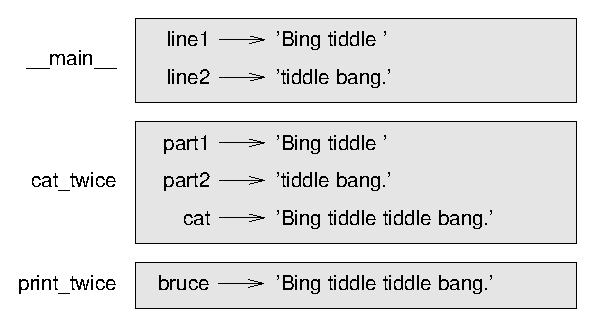
\includegraphics{figs/stack.eps}}
\afterfig

The frames are arranged in a stack that indicates which function
called which, and so on.  In this example, \verb"print_twice"
was called by \verb"cat_twice", and \verb"cat_twice" was called by 
\verb"__main__", which is a special name for the topmost frame.  When
you create a variable outside of any function, it belongs to 
\verb"__main__".

Each parameter refers to the same value as its corresponding
argument.  So, {\tt part1} has the same value as
{\tt line1}, {\tt part2} has the same value as {\tt line2},
and {\tt bruce} has the same value as {\tt cat}.

If an error occurs during a function call, Python prints the
name of the function, and the name of the function that called
it, and the name of the function that called {\em that}, all the
way back to \verb"__main__".

For example, if you try to access {\tt cat} from within 
\verb"print_twice", you get a {\tt NameError}:

\beforeverb
\begin{verbatim}
Traceback (innermost last):
  File "test.py", line 13, in __main__
    cat_twice(line1, line2)
  File "test.py", line 5, in cat_twice
    print_twice(cat)
  File "test.py", line 9, in print_twice
    print cat
NameError: name 'cat' is not defined
\end{verbatim}
\afterverb
%
This list of functions is called a {\bf traceback}.  It tells you what
program file the error occurred in, and what line, and what functions
were executing at the time.  It also shows the line of code that
caused the error.

\index{traceback}

The order of the functions in the traceback is the same as the
order of the frames in the stack diagram.  The function that is
currently running is at the bottom.


\section{Boolean functions}
\label{boolean}

\index{boolean function}

Functions can return booleans, which is often convenient for hiding
complicated tests inside functions.  For example:

\beforeverb
\begin{verbatim}
def is_divisible(x, y):
    if x % y == 0:
        return True
    else:
        return False
\end{verbatim}
\afterverb
%
It is common to give boolean functions names that sound like yes/no
questions; \verb"is_divisible" returns either {\tt True} or {\tt False}
to indicate whether {\tt x} is divisible by {\tt y}.

Here is an example:

\beforeverb
\begin{verbatim}
>>>   is_divisible(6, 4)
False
>>>   is_divisible(6, 3)
True
\end{verbatim}
\afterverb
%
The result of the {\tt ==} operator is a boolean, so we can write the
function more concisely by returning it directly:

\beforeverb
\begin{verbatim}
def is_divisible(x, y):
    return x % y == 0
\end{verbatim}
\afterverb
%
Boolean functions are often used in conditional statements:

\index{conditional statement}
\index{statement!conditional}

\beforeverb
\begin{verbatim}
if is_divisible(x, y):
    print 'x is divisible by y'
\end{verbatim}
\afterverb
%
It might be tempting to write something like:

\beforeverb
\begin{verbatim}
if is_divisible(x, y) == True:
    print 'x is divisible by y'
\end{verbatim}
\afterverb
%
But the extra comparison is unnecessary.

\begin{ex}
Write a function \verb"is_between(x, y, z)" that
returns {\tt True} if $x \le y \le z$ or {\tt False} otherwise.
\end{ex}

% TBD - May want ot talk about "guarding" code here - lots removed

\section{Debugging}
\label{factdebug}

\index{debugging}

Breaking a large program into smaller functions creates natural
checkpoints for debugging.  If a function is not working, there are
three possibilities to consider:

\begin{itemize}

\item There is something wrong with the arguments the function
is getting; a precondition is violated.

\item There is something wrong with the function; a postcondition
is violated.

\item There is something wrong with the return value or the
way it is being used.

\end{itemize}

To rule out the first possibility, you can add a {\tt print} statement
at the beginning of the function and display the values of the
parameters (and maybe their types).  Or you can write code
that checks the preconditions explicitly.

\index{precondition}
\index{postcondition}

If the parameters look good, add a {\tt print} statement before each
{\tt return} statement that displays the return value.  If
possible, check the result by hand.  Consider calling the
function with values that make it easy to check the result
(as in Section~\ref{incremental development}).

If the function seems to be working, look at the function call
to make sure the return value is being used correctly (or used
at all!).

\index{flow of execution}

Adding print statements at the beginning and end of a function
can help make the flow of execution more visible.

If you are confused about the flow of execution, this kind of
output can be helpful.  It takes some time to develop effective
scaffolding, but a little bit of scaffolding can save a lot of debugging.


\section{Glossary}

\begin{description}

\item[temporary variable:]  A variable used to store an intermediate value in
a complex calculation.
\index{temporary variable}
\index{variable!temporary}

\item[dead code:]  Part of a program that can never be executed, often because
it appears after a {\tt return} statement.
\index{dead code}

\item[{\tt None}:]  A special value returned by functions that
have no return statement or a return statement without an argument.
\index{None special value}
\index{special value!None}

\item[local variable:]  A variable defined inside a function.  A local
variable can only be used inside its function.
\index{local variable}

\item[global variable:]  A variable defined outside a function.  Global
variables can be accessed from any function.
\index{global variable}

\item[declaration:] A statement like {\tt global} that tells the
interpreter something about a variable.
\index{declaration}


\item[incremental development:]  A program development plan intended to
avoid debugging by adding and testing only
a small amount of code at a time.
\index{incremental development}

\item[scaffolding:]  Code that is used during program development but is
not part of the final version.
\index{scaffolding}

\item[guardian:]  A programming pattern that uses a conditional
statement to check for and handle circumstances that
might cause an error.
\index{guardian pattern}
\index{pattern!guardian}

\item[stack diagram:]  A graphical representation of a stack of functions,
their variables, and the values they refer to.
\index{stack diagram}

\item[frame:]  A box in a stack diagram that represents a function call.
It contains the local variables and parameters of the function.
\index{function frame}
\index{frame}

\item[call graph:] A diagram that shows every frame created during
the execution of a program, with an arrow from each caller to
each callee. 

\index{call graph}
\index{diagram!call graph}

\item[traceback:]  A list of the functions that are executing,
printed when an exception occurs.
\index{traceback}

\item[flag:] A boolean variable used to indicate whether a condition
is true.
\index{flag}


\end{description}


\section{Exercises}

\begin{ex}
\index{stack diagram}

Draw a stack diagram for the following
program.  What does the program print?

\beforeverb
\begin{verbatim}
def b(z):
    prod = a(z, z)
    print z, prod
    return prod

def a(x, y):
    x = x + 1
    return x * y

def c(x, y, z):
    sum = x + y + z
    pow = b(sum)**2
    return pow

x = 1
y = x + 1
print c(x, y+3, x+y)
\end{verbatim}
\afterverb

\end{ex}



\begin{ex}
\label{palindrome}

\index{palindrome}

A palindrome is a word that is spelled the same backward and
forward, like ``noon'' and ``redivider''.  Recursively, a word
is a palindrome if the first and last letters are the same
and the middle is a palindrome.

The following are functions that take a string argument and
return the first, last, and middle letters:

\beforeverb
\begin{verbatim}
def first(word):
    return word[0]

def last(word):
    return word[-1]

def middle(word):
    return word[1:-1]
\end{verbatim}
\afterverb
%
We'll see how they work in Chapter~\ref{strings}.

\begin{enumerate}

\item Type these functions into a file named {\tt palindrome.py}
and test them out.  What happens if you call {\tt middle} with
a string with two letters?  One letter?  What about the empty
string, which is written \verb"''" and contains no letters?

\item Write a function called \verb"is_palindrome" that takes
a string argument and returns {\tt True} if it is a palindrome
and {\tt False} otherwise.  Remember that you can use the
built-in function {\tt len} to check the length of a string.

\end{enumerate}

\end{ex}

\begin{ex}
A number, $a$, is a power of $b$ if it is divisible by $b$
and $a/b$ is a power of $b$.  Write a function called
\verb"is_power" that takes parameters {\tt a} and {\tt b}
and returns {\tt True} if {\tt a} is a power of {\tt b}.
\end{ex}


\begin{ex}

\index{greatest common divisor (GCD)}
\index{GCD (greatest common divisor)}

The greatest common divisor (GCD) of $a$ and $b$ is the largest number
that divides both of them with no remainder\footnote{This exercise is
  based on an example from Abelson and Sussman's {\em Structure and
    Interpretation of Computer Programs}.}.

One way to find the GCD of two numbers is Euclid's algorithm,
which is based on the observation that if $r$ is the remainder
when $a$ is divided by $b$, then $gcd(a, b) = gcd(b, r)$.
As a base case, we can consider $gcd(a, 0) = a$.

\index{Euclid's algorithm}
\index{algorithm!Euclid}

Write a function called
\verb"gcd" that takes parameters {\tt a} and {\tt b}
and returns their greatest common divisor.  If you need
help, see \url{wikipedia.org/wiki/Euclidean_algorithm}.

\end{ex}





\chapter{Networked programs}

While many of the examples in this book have focused on reading
files and looking for data in those files, there are many different
sources of information when one considers the Internet.

In this chapter we will pretend to be a web browser and retrieve web
pages using the HyperText Transport Protocol (HTTP).  Then we will read
through the web page data and parse it.

\section{HyperText Transport Protocol - HTTP}

The network protocol that powers the web is actually quite simple and 
there is built-in support in Python called {\tt sockets} which makes it very 
easy to make network connections and retrieve data over those
sockets in a Python program.

A socket is much like a file, except that it provides a two-way connection between two 
programs with a single socket.  
You can both read from and write to the same socket.  If you write somthing to 
a socket is is sent to the application at the other end of the socket.  If you 
read from the socket, you are given the data which the other application has sent.

But if you try to read a socket when the program on the other end of the socket
has not sent any data - you just sit and wait.  And if the programs on both ends
of the socket simply wait for some data without sending anything, they will wait for
a very long time.

So an important part of programs which communicate over the Internet is to have some
sort of protocol.   A protocol is a set of precise rules that determine who
is to go first, what they are to do, and then what are the responses to that message,
and who sends next and so no.  In a sense the two applications at either end 
of the socket are doing a dance and making sure not to step on each other's toes.

There are many documents which describe these network protocols.  The HyperText Transport 
Protocol is described in the following document:

\url{http://www.w3.org/Protocols/rfc2616/rfc2616.txt}

This is a long and complex 176 page document with a lot of detail.  If you 
find it interesting feel free to read it all.  But if you take a look around page 36 of
RFC2616 you will find the syntax for the GET request.  If you read in detail, you will
find that to reqest a document from a web server, we make a connection to 
the {\tt www.py4inf.com} server on port 80, and then send a line of the form:

{\tt GET http://www.py4inf.com/code/romeo.txt HTTP/1.0 }

Where the second parameter is the web page we are requesting and then 
we also send a blank line.  The web server will respond with some 
header information about the document and a blank line
followed by the document content.

\section{The World's Simplest Web Browser}

Perhaps the easiest way to show how the HTTP protocol works is to write a very 
simple Python program that makes a connection to a web server and following
the rules of the HTTP protocol, requests a document 
and displays what the server sends back.

\beforeverb
\begin{verbatim}
import socket

mysock = socket.socket(socket.AF_INET, socket.SOCK_STREAM)
mysock.connect(("www.py4inf.com", 80))
mysock.send("GET http://www.py4inf.com/code/romeo.txt HTTP/1.0\n\n")

while True:
    data = mysock.recv(512)
    if ( len(data) < 1 ) :
        break
    print data

mysock.close()
\end{verbatim}
\afterverb
%
First the program makes a connection to port 80 on 
the server www.py4inf.com.
Since our program is playing the role of the "web browser" the HTTP
protocol says we must send the GET command followed by a blank line.

Once we send that blank line, we write a loop that receives data 
in 512 character chunks from the socket and prints the data out 
until there is no more data to read (i.e. the recv() returns 
an empty string).

The program prodces the following output:

\beforeverb
\begin{verbatim}
HTTP/1.1 200 OK
Date: Sun, 14 Mar 2010 23:52:41 GMT
Server: Apache
Last-Modified: Tue, 29 Dec 2009 01:31:22 GMT
ETag: "143c1b33-a7-4b395bea"
Accept-Ranges: bytes
Content-Length: 167
Connection: close
Content-Type: text/plain

But soft what light through yonder window breaks
It is the east and Juliet is the sun
Arise fair sun and kill the envious moon
Who is already sick and pale with grief
\end{verbatim}
\afterverb
%
The output starts with headers which the web server sends
to describe the document.
For example, the {\tt Content-Type } header indicated that
the document is a plain text document ({\tt text/plain}).

After the server sends us the headers, it adds a blank line
to indicate the end of the headers and then sends the actual
data of the file {\tt romeo.txt}.

This example shows how to make a low-level network connection
with sockets.   Sockets can be use to communicate with a web
server or with a mail server or many kineds of servers.
All that is needed is to find the document shich describes
the protocol and rite code to send and receive the data
according to the protocol.

However since the protocol that we use most commonly is
the HTTP (i.e. the web) protocol, Python has a special 
library specifically designed to support the HTTP protocol 
for retrieval of
documents and data over the web.

\section{Retrieving web pages with {\tt urllib}}

The {\tt urllib} library makes it very easy to retrieve
web pages and process the data in Python.   Using {\tt urllib}
you can treat a web page much like a file.   You simply
indiate which web page you would like to retrieve and
{\tt urllib} handles all of the HTTP protocol details.

The equivalent code to read the {\tt romeo.txt} file
from the web using {\tt urllib} is as follows:

\beforeverb
\begin{verbatim}
import urllib

fhand = urllib.urlopen('http://www.py4inf.com/code/romeo.txt')
for line in fhand:
   print line.strip()
\end{verbatim}
\afterverb
%
Once the web page has been openned with 
{\tt urllib.urlopen} we can treat it like 
a file and read through it using a 
{\tt for} loop.   

When the program runs, we only see the output
of the contents of the file.   The headers
are still sent, but the {\tt urllib} code
consumes the headers and only returns the 
data to us.

\beforeverb
\begin{verbatim}
But soft what light through yonder window breaks
It is the east and Juliet is the sun
Arise fair sun and kill the envious moon
Who is already sick and pale with grief
\end{verbatim}
\afterverb
%

As an example, we can write 
a program to retrieve the data for
{\tt romeo.txt} and compute the frequency
of each word in the file as follows:

\beforeverb
\begin{verbatim}
import urllib

counts = dict()
fhand = urllib.urlopen('http://www.py4inf.com/code/romeo.txt')
for line in fhand:
   words = line.split()
   for word in words:
      counts[word] = counts.get(word,0) + 1   
print counts
\end{verbatim}
\afterverb
%
Again, once we have opened the web page, 
we can read it like a local file.

\section{Parsing HTML and scraping the web}

One of the common uses of the {\tt urllib} capability in Python is 
to "scrape" the web.   Web scraping is when we write a program
that pretends to be a web browser and retrieves pages and then 
examines the data in those pages looking for patterns.

As an example, a search engine such as Google will look at source 
of one web page and extract the links to other pages and retrieve
those pages, extracting links, and so on.   Using this technique,
Google ``spiders'' its way through nearly all of the pages on 
the web.   
Google also uses the frequency of links from pages it finds 
to a particular page as one measure of how ``important'' 
a page is and how highly the page should appear in its search results.

There are a number of Python libraries which can help you parse
HTML and extract data from the pages.  Each of the libraries
has its strengths and weaknesses and you can pick one based on 
your needs.

As an example, we will simply parse some HTML input 
and extract links using Python string functions.   Here is a 
simple web page:

\beforeverb
\begin{verbatim}
<h1>The First Page</h1>
<p>
If you like, you can switch to the
<a href="http://www.dr-chuck.com/page2.htm">
Second Page</a>.
</p>
\end{verbatim}
\afterverb
%
We will read through the page and key off the ``href'' string
in the line.   We will then use simple string manipulation
to  extract the information between the double quotes as follows:

\beforeverb
\begin{verbatim}
import urllib

url = raw_input('Enter - ')
fhand = urllib.urlopen(url)
for line in fhand:
   pos = line.find('href="')
   if pos < 1 : continue
   rest = line[pos+6:]
   end = rest.find('"')
   if end < 1 : continue
   link = rest[:end]
   print link
\end{verbatim}
\afterverb
%
The program prompts for a web address, then opens the web
address and starts looping through the lines of the web page.
First it loks for lines with ``href'' and skips the lines
that do not have the ``href'' string.  On lines with the 
``href'' string, the code skips past the ``href'', equals sign, 
and double quote and takes the rest of the line.

It then searches for the next double quote in the rest of the 
line and treats the link as the text up to but not 
including the second double quote.

When the program is run it looks as follows:

\beforeverb
\begin{verbatim}
python urllinks.py 
Enter - http://www.dr-chuck.com/page1.htm
http://www.dr-chuck.com/page2.htm

python urllinks.py 
Enter - http://www.py4inf.com/
/glike.css
py4inf_cover.jpg
http://www.greenteapress.com/thinkpython/thinkpython.html
http://allendowney.com/
http://www.si502.com/
http://www.lib.umich.edu/espresso-book-machine
http://www.py4inf.com/code
http://www.pythonlearn.com/
\end{verbatim}
\afterverb
%
\section{Glossary}

\begin{description}

\item[port:] A number that generally indicates which application 
you are contacting when you make a socket connection to a server.
As an example, web traffic usually uses port 80 while e-mail 
traffic uses port 50.
\index{port}

\item[scrape:] When a program pretends to be a web browser and
retrives a web page and then lokas at the web page content. 
Often programs are following the links in one page to find the next
page so they can traverse a network of pages or a social network.
\index{socket}

\item[socket:] A network connection between two applications
where the appcliations can send and receive data in either direction.
\index{socket}

\item[spider:] The act of a web search engine retrieving a page and
then all the pages linked from a page and so on until they have 
nealry all of the pages on the Internet which they 
use to build their search index.
\index{spider}

\end{description}

\section{Exercises}

\begin{ex}
Download the Google Application Engine Python SDK from 

\url{http://code.google.com/appengine/downloads.html}

And create the ``hello world'' application and get it up and running
on your computer.  Then adapt the simple {\tt socket} program to 
connect to your web server running at {\tt http://localhost:8080/}
instead of {\tt http://www.py4inf.com/code/romeo.txt}.  Remember that
the ``8080'' is the non-default HTTP port number while 80 is the 
default http port number.

The output should look as follows:
\beforeverb
\begin{verbatim}
HTTP/1.0 200 Good to go

Server: Development/1.0
Date: Wed, 17 Mar 2010 20:30:59 GMT
Content-Type: text/plain
Cache-Control: no-cache
Expires: Fri, 01 Jan 1990 00:00:00 GMT
Content-Length: 17

Hello there Chuck
\end{verbatim}
\afterverb
%
\end{ex}

\begin{ex}
Change the program which uses {\tt urllib} and reads and prints
the data to talk to your web server running at 
{\tt http://localhost:8080/}.
How is the ouput different from the previous exercise and why?
\end{ex}


\chapter{Using Web Services}

Once it became easy to retrieve documents and parse documents 
over HTTP using programs, it did not take long to develop 
an approach where we started producing documents that were specifically
designed to be consumed by other programs instead docuents
intended to be viewed in a browser using HyperText Markup Language
(HTML).

The most common approach when two programs are exchanging data across 
the web is to exchange the data in a format called the ``eXtensible Markup 
Language'' or XML.  

\section{eXtensible Markup Language - XML}

XML looks very similar to HTML, but XML is more structured 
than HTML.  Here is a sample of an XML document:

\beforeverb
\begin{verbatim}
<person>
  <name>Chuck</name>
  <phone type="intl">
     +1 734 303 4456
   </phone>
   <email hide="yes"/>
</person>
\end{verbatim}
\afterverb
%
\section{Parsing XML}

Here is a simple application that parses some XML
and extracts some data elements from the XML:

\beforeverb
\begin{verbatim}
import xml.etree.ElementTree as ET

data = '''
<person>
  <name>Chuck</name>
  <phone type="intl">
     +1 734 303 4456
   </phone>
   <email hide="yes"/>
</person>'''

tree = ET.fromstring(data)
print 'Name:',tree.find('name').text
print 'Attr:',tree.find('email').get('hide')
\end{verbatim}
\afterverb
%
The call to {\tt fromstring} converts the string representation
of the XML into a 'tree' of XML Elements.  When the
XML is in a tree, we have a seties of methods which we can call to 
extract portions of data from the XML.  

The {\tt find} function searches through the 
XML tree and retrieves a {\bf node} that matches the specified tag.
Each node can have some text, some attributes (i.e. like hide) and
some ``child'' nodes.   Each node can be the top of a tree of nodes.

\beforeverb
\begin{verbatim}
Name: Chuck
Attr: yes
\end{verbatim}
\afterverb
%
Using an XML parser such as {\tt ElementTree} has the advantage
in that while the XML in this example is quite simple, it turns
out that there are many rules regarding valid XML and using 
{\tt ElementTree} allows us to extract data from XML without 
worrying about the rules of XML syntax.

\section{Looping through nodes}

Often the XML has multiple nodes and we need to write a loop
to process all of the nodes.  In the following program, 
we loop through all of the {\tt user} nodes:

\beforeverb
\begin{verbatim}
import xml.etree.ElementTree as ET

input = '''
<stuff>
    <users>
        <user x="2">
            <id>001</id>
            <name>Chuck</name>
        </user>
        <user x="7">
            <id>009</id>
            <name>Brent</name>
            </user>
        </users>
</stuff>'''

stuff = ET.fromstring(input)
lst = stuff.findall("users/user")
print 'User count:', len(lst)

for item in lst:
    print 'Name', item.find('name').text
    print 'Id', item.find('id').text
    print 'Attribute', item.get("x")
\end{verbatim}
\afterverb
%
The {\tt findall} method retrieves a Python list of sub-trees that
represent the {\tt user} structures in the XML tree.  Then we can 
write a {\tt for} loop that looks at each of the user nodes, and 
prints the {\tt name} and {\tt id} text elements as well as the 
{\tt x} attribute from the user node.

\beforeverb
\begin{verbatim}
User count: 2
Name Chuck
Id 001
Attribute 2
Name Brent
Id 009
Attribute 7
\end{verbatim}
\afterverb
%

\section{Application Programming Interfaces (API)}

We now have the ability to exchange data between applications using HyperText
Transport Protocol (HTTP) and a way to represent complex data that we are 
sending back and forth between these applications using eXtensible 
Markup Language (XML).

The next step is to begin to define and document ``contracts'' between 
applications usig these techniques. The general name for these 
application-to-application contracts is {\bf Application Program 
Interfaces} or APIs.  When we use an API, generally one program
makes a set of {\bf services} available for use by other applications
and publishes the APIs (i.e. the ``rules'') which must be followed to 
access the services provided by the program.

When we begin to build our programs where the functionality of
our program includes access to services provided by other programs, 
we call the approach a {\bf Service-Oriented Architecture} or SOA.
An SOA approach is one where our overall application makes use of 
the services of other applications.  A non-SOA approach is where the
application is a single stand-alone application which contains all of the
code necessary to implement the application.

We see many examples of SOA when we use the web.  We can go to a single 
web site and book air travel, hotels, and automobiles all from a 
single site.  The data for hotels is not stored on the airline computers. 
Instead, the airline computers contact the services on the hotel computers
and retrieve the hotel data and present it to the user.  When the user
agrees to make a hotel reservation using the airline site, the airline site uses
another web service on the hotel systems to actually make the reservation.
And when it comes to charge your credit card for the whole transaation, 
still other computers become involved in the process.

A Servce-Oriented Architecture has many advantages including: (1) we 
always maintain only one copy of data - this is particularly important
for things like hotel reservations where we do not want to over-commit
and (2) the owners of the data can set the rules about the use of their 
data.   With these advantages, a SOA system must be carefully designed
to have good performance and meet the user's needs.

When an application makes a set of services in its API available over the web, 
we call these {\bf web services}. 

\section{Twitter web services}

Many of you many be familiar with the Twitter web site and many Twitter
applications \url{http://www.twitter.com}.  Twitter has a very unique
approach to its API/web services in that all of its data is available
to non-Twitter applications using the Twitter API.

Because Twitter has been so liberal in allowing access to its data,
it has enabled thousands of software developers to build their own
customized Twitter-based software.  These additional applications greatly
increase the value of Twitter far beyond simply a web-site.  The 
Twitter web services allow the building of whole new applications that
the Twitter team may never of thought of.  It is said that over 90 percent
of the use of Twitter is through the API (i.e. not through the {\tt twitter.com}
web user inteface).

You can view the Twitter API documentation at 
\url{http://apiwiki.twitter.com/}.  We will focus on the API
to retrieve a list of a user's friends and their statuses.  As an 
example, you can visit the following URL:

\url{http://api.twitter.com/1/statuses/friends/drchuck.xml}

To see a list of the friends of the twitter account {\tt drchuck}.
It may look like a mess in your browser.   To see the actual XML
returned by Twitter, you can view the source of the returned
``web page''.

We can retrieve this same XML using Python using the {\tt urllib}
utility:

\beforeverb
\begin{verbatim}
import urllib

TWITTER_URL = 'http://api.twitter.com/l/statuses/friends/ACCT.xml'

while True:
    print ''
    acct = raw_input('Enter Twitter Account:')
    if ( len(acct) < 1 ) : break
    url = TWITTER_URL.replace('ACCT', acct)
    print 'Retrieving', url
    document = urllib.urlopen (url).read()
    print document[:250]
\end{verbatim}
\afterverb
%
The program prompts for a Twitter account and opens the URL
for the friends and statuses API and then retrieves the 
text from the URL and shows us the first 250 characters of
the text.

\beforeverb
\begin{verbatim}
python twitter1.py

Enter Twitter Account:drchuck
Retrieving http://api.twitter.com/l/statuses/friends/drchuck.xml
<?xml version="1.0" encoding="UTF-8"?>
<users type="array">
<user>
  <id>115636613</id>
  <name>Steve Coppin</name>
  <screen_name>steve_coppin</screen_name>
  <location>Kent, UK</location>
  <description>Software developing, best practicing, agile e

Enter Twitter Account:
\end{verbatim}
\afterverb
%
In this application, we have retrieved the XML exactly as if it were
an HTML web page.  If we wanted to extract data from the XML, we 
could use Python string functions but this would become pretty complex
as we tried to really start to dig into the XML in detail.

If we were to dump out some of the retrieved XML it would look roughly as follows:

\beforeverb
\begin{verbatim}
<?xml version="1.0" encoding="UTF-8"?>
<users type="array">
  <user>
    <id>115636613</id>
    <name>Steve Coppin</name>
    <screen_name>steve_coppin</screen_name>
    <location>Kent, UK</location>
    <status>
      <id>10174607039</id>
      <source>web</source>
      </status>
  </user>
  <user>
    <id>17428929</id>
    <name>davidkocher</name>
    <screen_name>davidkocher</screen_name>
    <location>Bern</location>
    <status>
      <id>10306231257</id>
      <text>@MikeGrace If possible please post a detailed bug report </text>
    </status>
  </user>
  ...
\end{verbatim}
\afterverb
%
The top level tag is a {\tt users} and there are multiple {\tt user} tags
below within the {\tt users} tag.   There is also a {\tt status} tag below
the {\tt user} tag.  

\section{Handling XML data from an API}

When we receive well-formed XML data from an API, we generally use
an XML parser such as {\tt ElementTree} to extract information from
the XML data.

In the program below, we retrieve the friends and statuses from
the Twitter API and then parse the returned XML to show the first
four friends and their statuses.

\beforeverb
\begin{verbatim}
import urllib
import xml.etree.ElementTree as ET

TWITTER_URL = 'http://api.twitter.com/l/statuses/friends/ACCT.xml'

while True:
    print ''
    acct = raw_input('Enter Twitter Account:')
    if ( len(acct) < 1 ) : break
    url = TWITTER_URL.replace('ACCT', acct)
    print 'Retrieving', url
    document = urllib.urlopen (url).read()
    print 'Retrieved', len(document), 'characters.' 
    tree = ET.fromstring(document)
    count = 0
    for user in tree.findall('user'):
        count = count + 1
        if count > 4 : break
        print user.find('screen_name').text
        status =  user.find('status')
        if status : 
            txt = status.find('text').text
            print '  ',txt[:50]
\end{verbatim}
\afterverb
%
We use the {\tt findall} method to get a list of the {\tt user} 
nodes and loop through the list using a {\tt for } loop.  
For each {\tt user} node, we pull out the text of the \verb"screen_name" node
and then pull out the {\tt status} node.   If there is a {\tt status}
node, we pull out the text of the {\tt text} node and print the first 50 
characters of the status text.

The pattern is pretty straightforward, we use {\tt findall} and {\tt find}
to pull out a list of nodes or a single node and then if a node is a complex
element with more sub-nodes we look deeper into the node until we reach the 
text element that we are interested in.

The program runs as follows:

\beforeverb
\begin{verbatim}
python twitter2.py 

Enter Twitter Account:drchuck
Retrieving http://api.twitter.com/l/statuses/friends/drchuck.xml
Retrieved 193310 characters.
steve_coppin
   Looking forward to some "oh no the markets closed,
davidkocher
   @MikeGrace If possible please post a detailed bug 
hrheingold
   From today's Columbia Journalism Review, on crap d
huge_idea
   @drchuck  #cnx2010 misses you, too.  Thanks for co

Enter Twitter Account:hrheingold
Retrieving http://api.twitter.com/l/statuses/friends/hrheingold.xml
Retrieved 208081 characters.
carr2n
   RT @tysone: Saturday's proclaimation by @carr2n pr
tiffanyshlain
   RT @ScottKirsner: Turning smartphones into a tool 
soniasimone
   @ACCompanyC Funny, smart, cute, and also nice! He 
JenStone7617
   Watching "Changing The Equation: High Tech Answers

Enter Twitter Account:
\end{verbatim}
\afterverb
%
While the code for parsig the XML and extracting the fields
using {\tt ElementTree} takes a few lines to express what 
we are looking for in the XML, it is much simpler than trying 
to use Python string parsing to pull apart the XML and find 
the data elements.

\section{Exercises}

\begin{ex}
Change the program that retrieves twitter data to also
print out the location for each of the friends
indented under the name by two spaces as follows:

\beforeverb
\begin{verbatim}
Enter Twitter Account:drchuck
Retrieving http://api.twitter.com/l/statuses/friends/drchuck.xml
Retrieved 194533 characters.
steve_coppin
   Kent, UK
   Looking forward to some "oh no the markets closed,
davidkocher
   Bern
   @MikeGrace If possible please post a detailed bug 
hrheingold
   San Francisco Bay Area
   RT @barrywellman: Lovely AmBerhSci Internet & Comm
huge_idea
   Boston, MA
   @drchuck  #cnx2010 misses you, too.  Thanks for co
\end{verbatim}
\afterverb
%
\end{ex}

\chapter{Using databases}

\section{What is a database?}
\index{database}

A {\bf database} is a file that is organized for storing data.
Most databases are organized like a dictionary in the sense
that they map from keys to values.  The biggest difference
is that the database is on disk (or other permanent storage),
so it persists after the program ends.

\index{anydbm module}
\index{module!anydbm}

The module {\tt anydbm} provides an interface for creating
and updating database files.  As an example, I'll create a database
that contains captions for image files.

\index{open function}
\index{function!open}

Opening a database is similar
to opening other files:

\beforeverb
\begin{verbatim}
>>> import anydbm
>>> db = anydbm.open('captions.db', 'c')
\end{verbatim}
\afterverb
%
The mode \verb"'c'" means that the database should be created if
it doesn't already exist.  The result is a database object
that can be used (for most operations) like a dictionary.
If you create a new item, {\tt anydbm} updates the database file.

\index{update!database}


\beforeverb
\begin{verbatim}
>>> db['cleese.png'] = 'Photo of John Cleese.'
\end{verbatim}
\afterverb
%
When you access one of the items, {\tt anydbm} reads the file:

\beforeverb
\begin{verbatim}
>>> print db['cleese.png']
Photo of John Cleese.
\end{verbatim}
\afterverb
%
If you make another assignment to an existing key, {\tt anydbm} replaces
the old value:

\beforeverb
\begin{verbatim}
>>> db['cleese.png'] = 'Photo of John Cleese doing a silly walk.'
>>> print db['cleese.png']
Photo of John Cleese doing a silly walk.
\end{verbatim}
\afterverb
%
Many dictionary methods, like {\tt keys} and {\tt items}, also
work with database objects.  So does iteration with a {\tt for}
statement.

\index{dictionary methods!anydbm module}

\beforeverb
\begin{verbatim}
for key in db:
     print key
\end{verbatim}
\afterverb
%
As with other files, you should close the database when you are
done:

\beforeverb
\begin{verbatim}
>>> db.close()
\end{verbatim}
\afterverb
%

\index{close method}
\index{method!close}


\section{Pickling}

\index{pickling}

A limitation of {\tt anydbm} is that the keys and values have
to be strings.  If you try to use any other type, you get an
error.

\index{pickle module}
\index{module!pickle}

The {\tt pickle} module can help.  It translates
almost any type of object into a string suitable for storage in a
database, and then translates strings back into objects.

{\tt pickle.dumps} takes an object as a parameter and returns
a string representation ({\tt dumps} is short for ``dump string''):

\beforeverb
\begin{verbatim}
>>> import pickle
>>> t = [1, 2, 3]
>>> pickle.dumps(t)
'(lp0\nI1\naI2\naI3\na.'
\end{verbatim}
\afterverb
%
The format isn't obvious to human readers; it is meant to be
easy for {\tt pickle} to interpret.  {\tt pickle.loads}
(``load string'') reconstitutes the object:

\beforeverb
\begin{verbatim}
>>> t1 = [1, 2, 3]
>>> s = pickle.dumps(t1)
>>> t2 = pickle.loads(s)
>>> print t2
[1, 2, 3]
\end{verbatim}
\afterverb
%
Although the new object has the same value as the old, it is
not (in general) the same object:

\beforeverb
\begin{verbatim}
>>> t1 == t2
True
>>> t1 is t2
False
\end{verbatim}
\afterverb
%
In other words, pickling and then unpickling has the same effect
as copying the object.

You can use {\tt pickle} to store non-strings in a database.
In fact, this combination is so common that it has been
encapsulated in a module called {\tt shelve}.  

\index{shelve module}
\index{module!shelve}


\begin{ex}

\index{anagram set}
\index{set!anagram}

If you did Exercise~\ref{anagrams}, modify your solution so that
it creates a database that maps from each word in the list to
a list of words that use the same set of letters.

Write a different program that opens the database and prints
the contents in a human-readable format.
\end{ex}



\section{Using the SQLite3 database}

\section{The basics of Structured Query Language (SQL)}

\section{Basic data modelling}

\section{Using JOIN to retrieve data}

\section{Python and SQLite3}

\chapter{Regular expressions}

\section{More accurate searching}

\section{Building regular expressions}

\section{Applications of regular expressions}

\section{Regular expressions at the command line (Advanced)}


\chapter{Automating common tasks}


\section{Filenames and paths}
\label{paths}

\index{filename}
\index{path}
\index{directory}
\index{folder}

Files are organized into {\bf directories} (also called ``folders'').
Every running program has a ``current directory,'' which is the
default directory for most operations.  
For example, when you open a file for reading, Python looks for it in the
current directory.

\index{os module}
\index{module!os}

The {\tt os} module provides functions for working with files and
directories (``os'' stands for ``operating system'').  {\tt os.getcwd}
returns the name of the current directory:

\index{getcwd function}
\index{function!getcwd}

\beforeverb
\begin{verbatim}
>>> import os
>>> cwd = os.getcwd()
>>> print cwd
/home/dinsdale
\end{verbatim}
\afterverb
%
{\tt cwd} stands for ``current working directory.''  The result in
this example is {\tt /home/dinsdale}, which is the home directory of a
user named {\tt dinsdale}.

\index{working directory}
\index{directory!working}

A string like {\tt cwd} that identifies a file is called a {\bf path}.
A {\bf relative path} starts from the current directory;
an {\bf absolute path} starts from the topmost directory in the
file system.

\index{relative path}
\index{path!relative}
\index{absolute path}
\index{path!absolute}

The paths we have seen so far are simple filenames, so they are
relative to the current directory.  To find the absolute path to
a file, you can use {\tt os.path.abspath}:

\beforeverb
\begin{verbatim}
>>> os.path.abspath('memo.txt')
'/home/dinsdale/memo.txt'
\end{verbatim}
\afterverb
%
{\tt os.path.exists} checks
whether a file or directory exists:

\index{exists function}
\index{function!exists}

\beforeverb
\begin{verbatim}
>>> os.path.exists('memo.txt')
True
\end{verbatim}
\afterverb
%
If it exists, {\tt os.path.isdir} checks whether it's a directory:

\beforeverb
\begin{verbatim}
>>> os.path.isdir('memo.txt')
False
>>> os.path.isdir('music')
True
\end{verbatim}
\afterverb
%
Similarly, {\tt os.path.isfile} checks whether it's a file.

{\tt os.listdir} returns a list of the files (and other directories)
in the given directory:

\beforeverb
\begin{verbatim}
>>> os.listdir(cwd)
['music', 'photos', 'memo.txt']
\end{verbatim}
\afterverb
%
To demonstrate these functions, the following example
``walks'' through a directory, prints
the names of all the files, and calls itself recursively on
all the directories.

\index{walk, directory}
\index{directory!walk}

\beforeverb
\begin{verbatim}
def walk(dir):
    for name in os.listdir(dir):
        path = os.path.join(dir, name)

        if os.path.isfile(path):
            print path
        else:
            walk(path)
\end{verbatim}
\afterverb
%
{\tt os.path.join} takes a directory and a file name and joins
them into a complete path.  

\begin{ex}
Modify {\tt walk} so that instead of printing the names of
the files, it returns a list of names.
\end{ex}

\begin{ex}
The {\tt os} module provides a function called {\tt walk}
that is similar to this one but more versatile.  Read
the documentation and use it to print the names of the
files in a given directory and its subdirectories.
\end{ex}


\section{Pipes}

\index{shell}
\index{pipe}

Most operating systems provide a command-line interface,
also known as a {\bf shell}.  Shells usually provide commands
to navigate the file system and launch applications.  For
example, in Unix, you can change directories with {\tt cd},
display the contents of a directory with {\tt ls}, and launch
a web browser by typing (for example) {\tt firefox}.

\index{ls (Unix command)}
\index{Unix command!ls}

Any program that you can launch from the shell can also be
launched from Python using a {\bf pipe}.  A pipe is an object
that represents a running process.

For example, the Unix command {\tt ls -l} normally displays the
contents of the current directory (in long format).  You can
launch {\tt ls} with {\tt os.popen}:

\index{popen function}
\index{function!popen}

\beforeverb
\begin{verbatim}
>>> cmd = 'ls -l'
>>> fp = os.popen(cmd)
\end{verbatim}
\afterverb
%
The argument is a string that contains a shell command.  The
return value is a file pointer that behaves just like an open
file.  You can read the output from the {\tt ls} process one
line at a time with {\tt readline} or get the whole thing at
once with {\tt read}:

\index{readline method}
\index{method!readline}
\index{read method}
\index{method!read}

\beforeverb
\begin{verbatim}
>>> res = fp.read()
\end{verbatim}
\afterverb
%
When you are done, you close the pipe like a file:

\index{close method}
\index{method!close}

\beforeverb
\begin{verbatim}
>>> stat = fp.close()
>>> print stat
None
\end{verbatim}
\afterverb
%
The return value is the final status of the {\tt ls} process;
{\tt None} means that it ended normally (with no errors).

\index{file!compression}
\index{compression!file}
\index{Unix command!gunzip}
\index{gunzip (Unix command)}

A common use of pipes is to read a compressed file incrementally;
that is, without uncompressing the whole thing at once.  The
following function takes the name of a compressed file as a
parameter and returns a pipe that uses {\tt gunzip} to decompress
the contents:

\beforeverb
\begin{verbatim}
def open_gunzip(filename):
    cmd = 'gunzip -c ' + filename
    fp = os.popen(cmd)
    return fp
\end{verbatim}
\afterverb
%
If you read lines from {\tt fp} one at a time, you never have
to store the uncompressed file in memory or on disk.

\section{Exercises}

\begin{ex}
\label{checksum}

\index{MP3}

In a large collection of MP3 files, there may be more than one
copy of the same song, stored in different directories or with
different file names.  The goal of this exercise is to search for
these duplicates.

\begin{enumerate}

\item Write a program that searches a directory and all of its
subdirectories, recursively, and returns a list of complete paths
for all files with a given suffix (like {\tt .mp3}).
Hint: {\tt os.path} provides several useful functions for
manipulating file and path names.

\index{duplicate}
\index{MD5 algorithm}
\index{algorithm!MD5}
\index{checksum}

\item To recognize duplicates, you can use a hash function that
reads the file and generates a short summary
of the contents.  For example,
MD5 (Message-Digest algorithm 5) takes an arbitrarily-long
``message'' and returns a 128-bit ``checksum.''  The probability
is very small that two files with different contents will
return the same checksum.

You can read about MD5 at \url{wikipedia.org/wiki/Md5}.  On
a Unix system you can use the program {\tt md5sum} and a pipe to
compute checksums from Python.

\index{pipe}

\end{enumerate}

\end{ex}



\chapter{Visualizing data}

\section{Simple graphics in Python}

\section{Python and spreadsheets}

\section{Using Google visualization}



